% !TEX root=ricardo_draft.tex
%%% TeX-master: "ricardo_draft"~\ref{figure.simple_models}
\begin{figure*}[th!]
\begin{center}
\vspace{-1ex}
\centerline{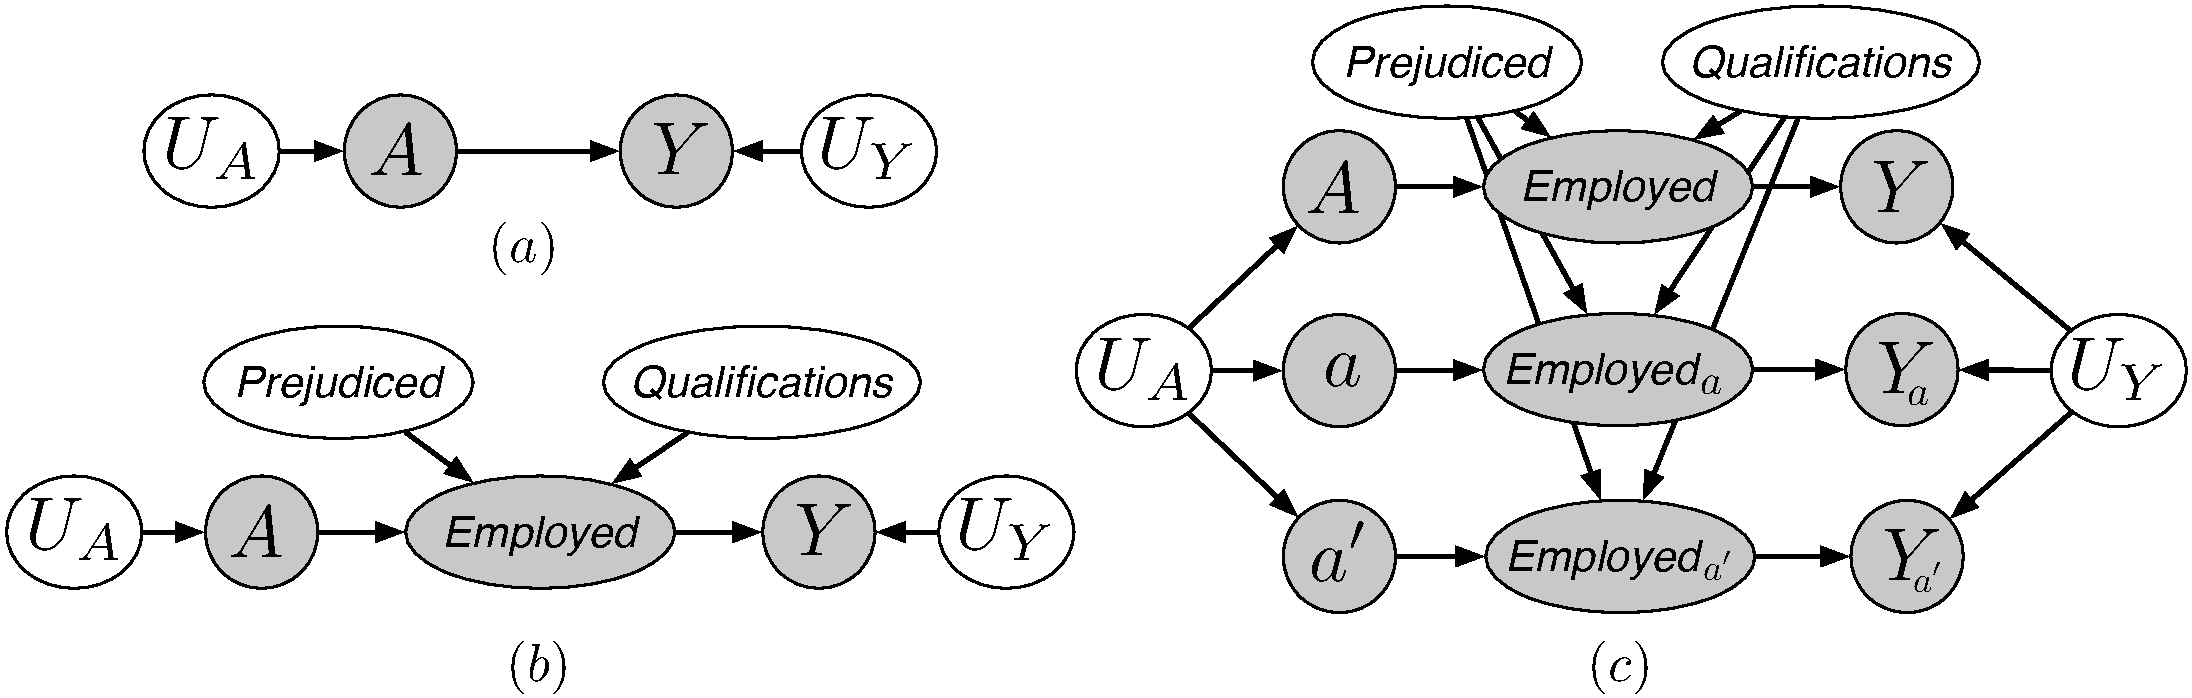
\includegraphics[width=\textwidth]{implications_fig.pdf}}
\vspace{-2ex}
\label{fig:ex1}
  \caption{(a) The graph corresponding to a causal model with $A$ being the protected attribute
    and $Y$ some outcome of interest, with background variables assumed to be independent.
    (b) Expanding the model to include an intermediate variable indicating whether the individual
    is employed with two (latent) background variables $\textbf{Prejudiced}$ (whether the person in charge
    of offering the job is prejudiced) and $\textbf{Qualifications}$ (a measure of the qualifications of
    the individual). (c) A twin network representation of this system \citep{pearl:00}
    under two different counterfactual levels for $A$. The network is created by creating copies
    of nodes descending from $A$, which inherit parents from the factual world that have not
    been affected.}
\vspace{-2ex}
\end{center}
% \begin{center}
  % \begin{tabular}{c}
  %   Here, a graph $U_A \rightarrow A \rightarrow Y \leftarrow U_Y$
  %   (rearrange it spatially in any way you want (including this table).)\\ (a)\\ \\
  %   Here, a graph made of edges \\
  %   $A \leftarrow U_A$, $Employed \leftarrow \{A, Prejudiced, Qualifications\}$,
  %   $Y \leftarrow \{Employed, U_Y\}$. \\ (b)\\ \\
  %   Here, a twin network,
  %   $A \leftarrow U_A$, $Employed \leftarrow \{A, Prejudiced, Qualifications\}$,
  %   $Y \leftarrow \{Employed, U_Y\}$,\\
  %   $Employed_a \leftarrow \{a, Prejudiced, Qualifications\}$,
  %   $Y_a \leftarrow \{Employed_a, U_Y\}$,\\
  %   $Employed_{a'} \leftarrow \{a', Prejudiced, Qualifications\}$,
  %   $Y_{a'} \leftarrow \{Employed_{a'}, U_Y\}$,
  %   (``$a$'' and ``$a'$'' are two extra nodes too)\\.
  %   \\ (c)\\
  % \end{tabular}
  % \label{fig:ex1}
  % \caption{(a) The graph corresponding to a causal model with $A$ being the protected outcome
  %   and $Y$ some outcome of interest, with background variables assumed to be independent.
  %   (b) Expanding the model to include an intermediate variable indicating whether the individual
  %   is employed with two (latent) background variables $\textbf{Prejudiced}$ (whether the person in charge
  %   of offering the job is prejudiced) and $\textbf{Qualifications}$ (a measure of the qualifications of
  %   the individual). (c) A twin network representation of this system \citep{pearl:00}
  %   under two different counterfactual levels for $A$. The network is created by creating copies
  %   of nodes descending from $A$, which inherit parents from the factual world that have not
  %   been affected.}
% \end{center}
\end{figure*}


\subsection{Definition}
%Formally, a variable $Y$ is said to be counterfactually fair with
%respect to a protected attribute $A$ if
Given a causal model $(U, V, F)$, let $A$ be a set of protected
attributes, $\hat Y$ a variable of interest which we will be the basis for

any decision making, and $W$ the set of complementary measurements such that
$W= V \setminus ( A \cup \{\hat Y\})$.
\begin{define}[Counterfactual fairness]
We say $\hat Y$ is {\bf counterfactually fair}
if under any context uniquely defined by $W = w$ and $A = a$,
  \label{eq:cf_definition}
\begin{align}
  &P(\hat Y_{A \leftarrow a\ }(U) = y\ |\ W = w, A = a)  =\nonumber\\ 
  &P(\hat Y_{A \leftarrow a'}(U) = y\ |\ W = w, A = a), 
\end{align}
for all $y$ and for any value $a'$ attainable by $A$.
\end{define}
Simply put,
the statement above captures the idea that any decision based on the
conditional distribution of $\hat Y$ would have been the same had $A$ been
different, given what has actually happened in the world.
We can also see $\hat Y$ as satisfying ``counterfactual exchangeability''
under this model.
%This definition substantially differs from Fairness Through
%Unawareness, as it considers the influence of attributes such as race
%on other measured variables.

An associated concept of causal fairness appears as Example 4.4.4 in
\citet{pearl:16}. There, the authors condition instead on $W$, $A$,
and the observed realization of $\hat Y$, and calculate the
probability of the counterfactual realization differing from the
factual\footnote{The result is an expression called the ``the
  probability of sufficiency'' for $A$, capturing the notion that
  switching $A$ to a different value would be sufficient to change
  $\hat Y$ with some probability.}. This example conflates the
recorded decision $\hat Y$ with the information $Y$ on which we should
ideally base our decision making, a difference which we maintain.  Our
framing makes the connection to other existing machine learning
methods more explicit, as we discuss in Section \ref{sec:methods}.
Evidence used to determine the state of background variables $U$
should come from $A$ and $W$ alone, as in many setups we wish to
predict some $Y$ as $\hat Y$, when $Y$ is unavailable at any point in
our inference.

We also emphasize that counterfactual fairness is an individual-level
definition. This is substantially different from the notion of ``causal independence''
as discussed in Section 4.3.1 of \cite{pearl:16}. Causal independence
% requires
% \begin{align}
%   &P(\hat Y = y\ |\ do(A = a), W = w) =\nonumber\\ 
%   &P(\hat Y = y\ |\ do(A = a'), W = w),
% \end{align}
% which
entails comparing different units that happen to share the
same ``treatment'' and coincide on values of $W$, while
counterfactual fairness concerns the variation possible within an
individual depending on their value of $a$ and the descendents of
$A$ in the causal graph.

\subsection{Implications}
%
As discussed by \citet{halpern:16}, it is unproductive to debate
if a particular counterfactual definition is the ``correct'' one
to satisfy socially constructed concepts such as blame and responsibility.
The same applies to fairness. Instead, we discuss the
implications of definition \eqref{eq:cf_definition} and some choices
that arise in its application.

First, we wish to make explicit the difference between $\hat Y$, the
variable which we use for fair decisions, and $Y$, the related state
generated by an unfair world. For instance, $Y$ could be an indicator
of whether a client defaults on a loan, while $\hat Y$ is the actual
decision of giving the loan. Consider the DAG $A \rightarrow Y$ for a
causal model where $V = \{A, Y\}$, and in Figure \ref{fig:ex1}(a) the
DAG with explicit inclusion of set $U$ and assumptions about
independence of background variables. Assume $Y$ is an objectively
ideal measure to be used in decision making, such as a binary
indicator that the individual defaults on a loan. In this setup, we
postulate that the mechanism $f_Y(A, U)$ is unfair, with the arrow
$A \rightarrow Y$ being the result of a world that punishes
individuals in a way that is out of their control. Figure
\ref{fig:ex1}(b) shows a more fine-grained theoretical model, where
the path is mediated by a measure of whether the person is employed,
which is itself caused by two background factors: one representing
whether the person offering jobs is prejudiced, and one related to
their qualifications. Using the information about employment will
result in unfair predictions if employment is partially the result of
prejudice.

In the world  postulated by this example 
$A$ is a cause of defaulting, even if mediated by other
variables. The counterfactual fairness principle however forbids us
from using $Y$: using the twin network construction of
\citet{pearl:00}, we see in Figure \ref{fig:ex1}(c) that $Y_a$ and
$Y_{a'}$ are not in general identically distributed given the
background variables.
  % \footnote{We assume
  % that function $f_Y(A, U)$ is not pathological, that is, it will give
  % different outcomes for different values of $A$ other things being
  % equal. Moreover, we assume interventions in $A$ are well defined.
  % For instance, ``race'' here could be formulated as ``race
  % perception'', which can be due to, for instance, to
  % racially-associated names in a C.V. or loan application.}
For example, if the function determining employment
$f_E(A,P,Q) = I_{(Q > 0, P = 0 \text{ or } A \neq a)}$ then an individual
with sufficient qualifications and prejudiced potential employer
may have a different counterfactual
employment value for $A = a$ compared to $A = a'$, and hence a
different probability of defaulting on a loan.


In contrast, any function of variables which are not descendants of
$A$ can be used a basis for fair decision making. This means, for instance,
that any variable $\hat Y$ defined by $\hat Y = g(U)$ will be counterfactually
fair for some arbitrary function $g(\cdot)$. Hence, given a causal
model, the functional defined by the function $g(\cdot)$ 
minimizing some predictive error for $Y$ will satisfy the criterion.
If for some reason $\hat Y$ needs to be randomized, it suffices that the
stochastic component of it is independent of any descendant of $A$.

% There are two issues to be clarified at this point. First,
% it sounds potentially counter-intuitive that our definition
% seemingly allows for the use of (background) variable $\textbf{Prejudiced}$
% directly. However, our point of view is that there is no harm: this is
% a feature of some other person who judged a job application of the
% individual concerned, not a feature of the individual. This variable
% might prove itself to be a useless predictor of $Y$ depending on the
% structural equations, resulting from the marginalization of $A$, but
% in principle it is not harmful as implied by the model.

% The second and more complicated issue concerns the fact that
There is a subtletly to address here: by abduction,
$U$ will typically depend on $A$, and hence so will $\hat Y$ when
marginalizing over $U$. This seems to disagree with the intuition that our
fair variable should be not be caused by $A$. We discuss
methods to address this in general in Section~\ref{sec:methods},
but consider the simple case where 
$U$ is fully determined by $A$ and $W$
(which occurs in some important special cases).
In this
scenario, we proceed just as if we have {\it measured} $U$ from the
beginning rather than performing abduction.
We then generate $\hat Y$ from $g(U)$, so $U$ is the cause of
$\hat Y$ and not $A$. 


% However, it appears to be the case that $\hat Y$ and $A$ will be
% ``causally dependent'' in general given $W$, meaning that $P(\hat Y =
% y\ |\ do(A = a), W = w) \neq P(\hat Y = y\ |\ do(A = a'), W = w)$.
% Our argument on why this is not a problem mirrors the discussion in
% Section 4.3.1 of \cite{pearl:16}, on the differences between
% counterfactual exchangeability and causal independence: the latter is
% a comparison among different units that happen to share the same
% treatment and coincide on the same outcomes for $W$. But in the
% postulated model $W$ responds to $A$ so, starting from a baseline
% individual with treatment $do(A = a)$ and measurements $w$, consider
% the generative model to generate a comparable individual: under $do(A
% = a')$, perform rejection sampling among individuals until we find
% someone who matches our target on the same $w$. This sampling
% mechanism gives a different posterior distribution for $U$ than the
% within-individual distribution\footnote{For example, if $w$ is a
%   common outcome under $do(A = a)$ and $P(U)$, but rare under $do(A =
%   a')$ and $P(U)$.} of the original individual, which is the one we care about in our
% definition. Hence, the inequality
% \begin{align}
%   P(\hat Y = y\ |\ do(A = a), W = w)
%   \neq P(\hat Y = y\ |\ do(A = a'), W = w)
% \end{align}
% should not be a matter of
% concern for a criterion defined for individual level differences.

It is important to note that we can build counterfactually fair
predictive models for some $Y$ even if the 
structural equations that generated $Y$ are unfair. The idea is that we
are learning a projection of $Y$ into an alternate world where it
would be fair, which we may think of as a
``closest world'' defined by our class of predictive models and the
causal structure of the world\footnote{The notion of ``closest world''
  is pervasive in the literature of counterfactual inference under
  different meanings \citep{pearl:00, halpern:16}.  Here, the cost
  function used to map fair variables to unfair outcomes also plays a
  role, but this concerns a problem dependent utility function that
  would be present anyway in the unfair prediction problem, and is
  orthogonal to the causal assumptions.}.




% TODO. Here the main
% definition is introduced, and how it relates to ``path deletion'',
% including the core example of $A \rightarrow X \rightarrow Y$, with
% two latent variables $U_x \rightarrow X$ and $U_y \rightarrow Y$,
% arguing that one might judge that the path from $A$ to $Y$ via is due
% to an unfair mechanism and that we need a notion of ``closest world''.


% When describing counterfactual fairness, it is important to
% distinguish between a counterfactually fair {\em world} in which the
% variable $Y$ we are interested in predicting is inherently
% counterfactually fair with respect to the protected attributes $A$,
% and a counterfactually fair {\em predictor} $\hat Y$, guaranteed to
% be counterfactually fair, regardless of the behavior of $Y$.

% Figure~\ref{figure.simple_models} shows possible worlds. {\em Left:} A
% counterfactually fair world in which the state of $Y$ has no
% dependencies on $A$. {\em Center and Right:} Potentially unfair worlds
% in which the state of $A$ can influence the state of $Y$ either
% indirectly as in {\em center} or directly as in {\em Right}.
\begin{figure*}[th]
\begin{center}
\vspace{-2ex}
\centerline{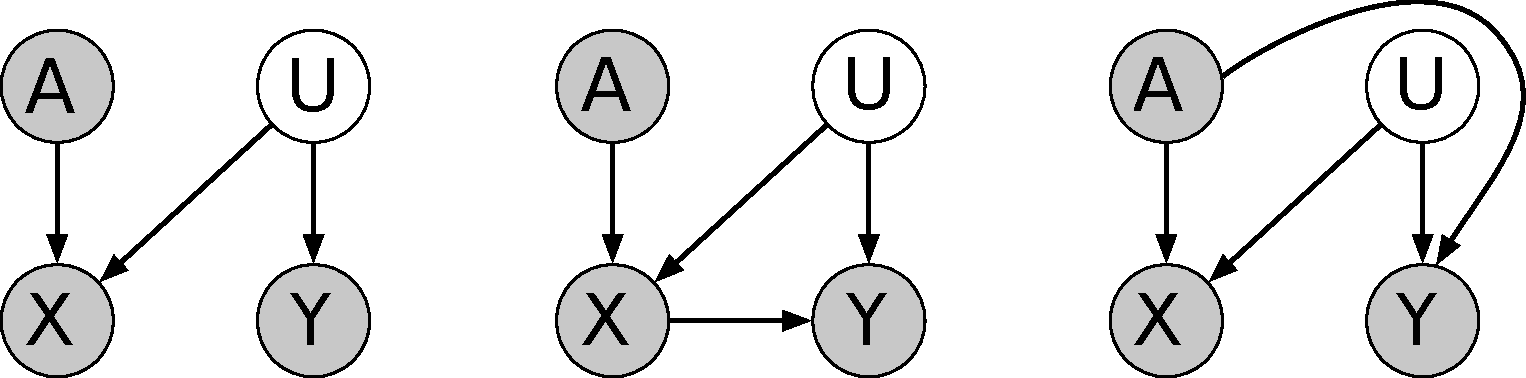
\includegraphics[width=0.9\textwidth]{simple_models_no_q2}}
\vspace{-2ex}
\caption{Three causal models for different real-world fair prediction scenarios.\label{figure.simple_models} See section \ref{sec:count_fair} for discussion.}
\vspace{-2ex}
\end{center}
\end{figure*}

\subsection{Examples}
To give an intuition for counterfactual fairness we will consider three % real-world
fair prediction scenarios: \textbf{insurance pricing}; \textbf{crime prediction}; \textbf{college admissions}. Each of these correspond to one of the three causal graphs in Figure~\ref{figure.simple_models}, and are discussed below.
%
\paragraph{Scenario 1: The Red Car.}
Imagine a car insurance company wishes to price insurance for car owners by
predicting their accident rate $Y$. They assume there is an
unobserved factor corresponding to aggressive driving $U$, that (a) causes
drivers to be more likely have an accident, and (b) causes individuals to prefer red cars (the observed
variable $X$). Moreover, individuals belonging to a
certain race $A$ are more likely to drive red cars. However, these individuals are no more likely to be aggressive or to get in accidents than any one else. We show this scenario in Figure~\ref{figure.simple_models} (\emph{Left}).

Thus, using the red car feature $X$ to predict accident likelihood $Y$
would seem to be an unfair prediction because it may charge
individuals of a certain race more than others, even though {\em no
  race is more likely to have an accident}. Counterfactual fairness
agrees with this notion.
%
\begin{lem}
The predictor $\hat{Y}(X)$ is not counterfactually fair for the model in Figure~\ref{figure.simple_models} (\emph{Left}).
\end{lem}
%
\begin{proof}
For simplicity, consider the case where the equations described by the model in Figure~\ref{figure.simple_models} (\emph{Left}) are deterministic and linear:
\begin{align}
X = \alpha A + \beta U, \;\;\;\; Y = \gamma U \nonumber
\end{align}
where the coefficients $\alpha,\beta,\gamma$ are given (in practice these are estimated), and by assumption $\alpha \neq 0$. We can test whether a predictor $\hat{Y}(X)$ is counterfactually-fair using the procedure described in Section~\ref{subsec:cmc}:
%\begin{itemize}
{\em (i)} Compute $U$ given observations of $X,Y,A$.%, by solving for $U$. 
{\em (ii)} Substitute the equations involving $A$ with an interventional value $a'$. 
% (i.e., this says: `what happens if the race of an individual were changed')
{\em (iii)} Compute the variables $X,Y$ with the interventional value $a'$.

In this deterministic case we achieve counterfactual fairness only if the predicted value $\hat{Y}(X)$ is identical before and after we change $A$. However, changing $A$ changes $X$. Thus $\hat{Y}(X)$ must be different and the model  is not counterfactually fair.
\end{proof}
The above result holds in a more general case: any non-constant estimator that depends only on a single $X$ is not be counterfactually fair as changing $A$ always alters $X$.
%
%
\paragraph{Scenario 2: High Crime Regions.} 
A local police precinct wants to know how likely a given house is to be broken into, $Y$. This likelihood depends on many unobserved factors
($U$) but also upon the neighborhood the house lies in ($X$). However, different ethnic groups are more likely to live in particular neighbourhoods, and so neighbourhood and break-in rates are often strongly correlated with the 
race $A$ of the house occupier. This scenario can be seen in Figure~\ref{figure.simple_models} (\emph{Center}).


% In such a scenario, although the likelihood of a particular
% person having their house broken into does not depend upon race
% directly, it does vary which a persons race and so is not
% counterfactually fair.

\paragraph{Scenario 3: University Success.}
A university wants to know if a student is likely to be successful after they graduate $Y$. They have information such as incoming grade point average (GPA), advanced placement (AP) exams results, and other academic features $X$. The university believes however, that an individual's gender may influence these features as well as their post-graduation success $Y$ due to social discrimination. Instead, they would like to model an individual's latent talent $U$ which causes $X$ and $Y$. We show this scenario in Figure~\ref{figure.simple_models} (\emph{Right}).

%  The world on the right shows $Y'$ a
% causally fair variable that doesn't depend on $A$ being directly
% corrupted by a bias relating to $A$, resulting in an observation
% $Y$. In this case, learning a causally fair approximation of $Y$ can
% recover the true variable $Y'$ (up to noise).


% \subsection{Examples}
% To get an intution for what the different definitions of fairness imply, we will
% revisit the examples of figure \ref{figure.simple_models}.
% begin by describing a few possible real-world scenarios. For each of these we will describe what counterfactually-fair and counterfactually-unfair predictors look like.

% \paragraph{Scenario 1: The Red Car.}
% Imagine a car insurance company wants a quick, anonymous way to determine how to price insurance for different car owners by predicting their accident likelihood $Y$. They've noticed that there is a correlation between driving a red car $X$ and a higher rate of automobile accidents. Thus they would like to increase the insurance for all red car drivers. 

% Imagine what's really going on is shown in Figure~\ref{figure.simple_models} (\emph{Left}). The correlation between have a red car $X$ and accidents $Y$ is due to an `aggressiveness' factor $U$: aggressiveness causes individuals to be in accidents more often, and it also attracts them to red cars. Unfortunately, the red car feature $X$ is also affected by an individual's race $A$. 

% TODO. Here the examples and their motivation can be as follows:

% \begin{itemize}
% \item something analogous to the red car example: $A$ is not a cause of
%   $Y$ but might indirectly bias the result even without using $A$ as a predictor;
% \item something with selection bias, maybe a toy version of COMPAS;
% \item something where an unfair judgment (say, credit score) that can be potentially
%   considered as a target variable, and an
%   ``objective target'' (say, defaulting on a loan) are present, and
%   what the recommendation is
% \end{itemize}
%%% Local Variables:
%%% mode: latex
%%% TeX-master: "ricardo_draft"
%%% End:
